\documentclass[conference]{IEEEtran}
\usepackage{amsmath,amssymb}
\usepackage{graphicx}
\usepackage{cite}
\usepackage{textcomp}
\usepackage{xcolor}
\usepackage{booktabs}
\usepackage{microtype}
\usepackage[colorlinks=true, linkcolor=blue, citecolor=blue, urlcolor=blue]{hyperref}

% Strict IEEE 6-page float and compaction controls
\setcounter{topnumber}{3}
\setcounter{bottomnumber}{3}
\setcounter{totalnumber}{6}
\setcounter{dbltopnumber}{2}
\renewcommand{\dbltopfraction}{0.95}
\renewcommand{\topfraction}{0.95}
\renewcommand{\bottomfraction}{0.90}
\renewcommand{\textfraction}{0.05}
\renewcommand{\floatpagefraction}{0.85}
\setlength{\textfloatsep}{5pt plus 1pt minus 1pt}
\setlength{\dbltextfloatsep}{5pt plus 1pt minus 1pt}
\setlength{\floatsep}{3pt plus 1pt minus 1pt}
\setlength{\dblfloatsep}{3pt plus 1pt minus 1pt}
\setlength{\intextsep}{3pt plus 1pt minus 1pt}

\begin{document}

\title{AI-ML Based Intelligent Dead Reckoning and 3D Map-Matching System for Seamless Navigation}

\author{
\IEEEauthorblockN{1\textsuperscript{st} Shreya Kesarwani}
\IEEEauthorblockA{\small Computer Science and Engineering\\
United College of Engineering \& Research\\
Prayagraj, India\\
kesarwanishreya2005@gmail.com}
\and
\IEEEauthorblockN{2\textsuperscript{nd} Akash Mishra}
\IEEEauthorblockA{\small Computer Science and Engineering\\
United College of Engineering \& Research\\
Prayagraj, India\\
akashmishra1910@gmail.com}
\and
\IEEEauthorblockN{3\textsuperscript{rd} Suchitra}
\IEEEauthorblockA{\small Computer Science and Engineering\\
United College of Engineering \& Research\\
Prayagraj, India\\
mesuchitradutta@gmail.com}
}

\maketitle

\begin{abstract}
Smartphone navigation systems are the primary positioning consoles for vehicular transit across dense corridors where Global Navigation Satellite System (GNSS) reception regularly degrades in tunnels, multi-level structures, and urban canyons. However, consumer smartphone MEMS inertial measurement units (IMUs) suffer from stochastic bias drift and severe road vibrations, causing unconstrained double-integration errors to accumulate by hundreds of meters within seconds. In this work, we propose an edge-deployable Intelligent Dead Reckoning (IDR) and 3D map-matching framework that operates framework-free on commodity smartphones without vehicle OBD-II telemetry. Following offline training in Python, the GBDT forward-velocity regressor and shock filter are compiled into native C++ decision tables that execute with zero external deep learning runtime dependencies. The system tightly couples dynamic gravity leveling, an in-vehicle cradle alignment watchdog, a 15-state Error-State Kalman Filter (ESKF) with data-driven Non-Holonomic Constraints (NHC) and Zero-Velocity Updates (ZUPT), and an elevation-aware 3D topological map-matcher. Evaluated on a high-fidelity trajectory emulation platform adhering to the IO-VNBD benchmark schema \cite{onyekpe2021} incorporating multi-driver naturalistic driving dynamics and road vibrations, all baseline models and proposed configurations are directly implemented and evaluated on identical tracks. On continuous cruising corridors, the proposed 15-state ESKF bounds drift to $2.01 \pm 0.18\%$ at 60\,s and $2.88 \pm 0.24\%$ at 120\,s, substantially outperforming directly re-run strapdown double integration (61.5\% at 60\,s) and open-loop AI velocity dead reckoning (27.9\% at 60\,s). Under urban stop-and-go outages with traffic halts, ZUPT actively reduces drift from 4.61\% to 2.58\% (a 44.0\% relative error reduction). Furthermore, the 3D map-matcher bounds full-system endpoint drift to 1.72\% (60\,s) and 2.80\% (120\,s) with 99.7\%--100\% flyover disambiguation accuracy at an end-to-end dead-reckoning cycle latency of $0.18 \pm 0.02$\,ms on mobile hardware.
\end{abstract}

\begin{IEEEkeywords}
dead reckoning, sensor fusion, GNSS-denied navigation, error-state Kalman filter, map matching, machine learning, non-holonomic constraints.
\end{IEEEkeywords}

\section{Introduction}

\subsection{Background}
Vehicle logistics, ride-hailing fleets, and emergency services rely heavily on smartphone navigation utilizing constellations such as GPS, Galileo, GLONASS, and NavIC. In emerging transport ecosystems such as India, smartphones mounted in commercial cradles serve as primary navigation consoles. These fleets lack factory-installed, wheel-odometry-coupled Inertial Navigation Systems (INS). Consequently, during GNSS outages in urban canyons, vehicular tunnels, and multi-tier flyovers, positioning diverges rapidly. In automotive navigation, a cumulative drift below 10\% of distance traveled constitutes the recognized operational tolerance to prevent false route recalculations before satellite re-acquisition.

Inertial dead reckoning (DR) provides self-contained positioning immune to satellite attenuation \cite{brossard2020, lawal2024}. However, consumer smartphone MEMS sensors exhibit stochastic bias drift and noise. Double integrating uncorrected accelerations causes error to accumulate quadratically. Furthermore, smartphones experience extraneous accelerations from engine idle vibrations (15--30\,Hz) and severe road surface irregularities (potholes and bumps) that do not reflect center-of-mass vehicular displacement.

\subsection{Problem Statement}
Two practical challenges prevent classical inertial DR on commodity smartphones:
\begin{enumerate}
\item \textbf{Absence of Direct Speedometer Telemetry}: Without vehicle OBD-II or CAN bus telemetry, forward speed must be inferred purely from noisy, gravitationally coupled accelerometer and gyroscope streams \cite{brossard2020, qian2025}.
\item \textbf{Arbitrary Orientation, Cradle Slip, and Road Shocks}: Smartphones are mounted without mechanical alignment to the vehicle chassis. Road vibrations and severe pothole shocks ($\le 3.2g$) rapidly corrupt integration. Sharp turns can cause cradle slip, destroying coordinate transformations unless re-calibrated in real time \cite{matos2025}.
\end{enumerate}

\subsection{Aim and Contributions}
This paper presents a complete, edge-deployable framework (Fig.~\ref{fig:overall_arch}) that maintains accurate, drift-bounded 3D vehicle positioning during extended GNSS outages without OBD-II telemetry. Following offline training, the GBDT forward-velocity regressor and shock filter are compiled into native C++ decision lookup tables executing with zero external deep learning runtime dependencies. The primary contributions are:
\begin{itemize}
\item An end-to-end IDR architecture integrating dynamic gravity leveling, longitudinal PCA alignment with a slip watchdog, a native C++ regularized GBDT velocity regressor \cite{friedman2001}, a 15-state ESKF with Non-Holonomic Constraints (NHC) \cite{dissanayake2001} and ZUPT \cite{foxlin2005}, and a 3D elevation-aware HMM map-matcher \cite{newson2009}.
\item A unified mathematical formulation linking coordinate transformations, machine learning pseudo-measurements, error-state propagation \cite{sola2017}, and probabilistic 3D Viterbi map matching.
\item Systematic empirical validation adhering to the IO-VNBD benchmark schema \cite{onyekpe2021} across continuous expressway cruising and dense urban stop-and-go corridors under realistic sensor noise and road shocks. Baseline methods \cite{dissanayake2001, brossard2020} are directly implemented and re-run on identical corridors, demonstrating ESKF continuous drift bounded to $2.01 \pm 0.18\%$ (60\,s) and $2.88 \pm 0.24\%$ (120\,s) on continuous cruising, an active $44.0\%$ drift reduction from ZUPT during urban stop-and-go halts, full-system endpoint drift bounded to $\le 2.80\%$, $99.7\%$--$100\%$ flyover disambiguation, and a single-epoch dead-reckoning cycle latency of $0.18 \pm 0.02$\,ms on mobile hardware.
\end{itemize}

\section{Related Work}

Dead reckoning and vehicular localization have evolved across strapdown inertial navigation \cite{dissanayake2001, foxlin2005}, machine learning state estimators \cite{brossard2020, lawal2024, qian2025, mamun2026}, and road-network map matching \cite{newson2009, javed2024, sundar2026}. Table~\ref{tab:litreview} summarizes relevant benchmarks, surveys \cite{deshmukh2025, mamun2026}, and sensor fault analyses \cite{matos2025}. Classical strapdown INS double-integrates specific force and angular rates, but MEMS biases cause rapid divergence unless aided by kinematic constraints like NHC \cite{dissanayake2001} and ZUPT \cite{foxlin2005}. Deep learning approaches estimate speed from IMU windows \cite{brossard2020, qian2025}, but heavy neural networks incur substantial mobile runtime latency. In map matching, classical 2D HMMs \cite{newson2009, javed2024, sundar2026} snap positions to road polylines, but fail to resolve multi-deck flyovers. To ensure fair comparison, all baseline models in Section~VI were directly re-run on identical tracks under identical sensor noise.

\begin{table*}[t]
\centering
\caption{Literature Review Summary and Research Gaps}
\label{tab:litreview}
\scriptsize
\renewcommand{\arraystretch}{0.92}
\setlength{\tabcolsep}{3pt}
\resizebox{\textwidth}{!}{%
\begin{tabular}{|c|l|p{4.5cm}|p{4.5cm}|p{4.5cm}|}
\hline
\textbf{Ref.} & \textbf{Author \& Year} & \textbf{Core Findings} & \textbf{Methodology} & \textbf{Identified Gaps} \\
\hline
\cite{onyekpe2021} & Onyekpe et al., 2021 & Released IO-VNBD benchmark containing multi-driver naturalistic driving IMU data. & Empirical vehicular data collection across diverse road conditions and drivers. & Benchmark dataset release only; proposes no self-contained navigation system. \\
\hline
\cite{lawal2024} & Lawal, 2024 & Neural models cut average positional drift by up to 40\% over pure inertial DR. & Contextual survey; RNN/LSTM sequence modeling. & Heavy compute overhead; lacks deterministic smartphone edge execution. \\
\hline
\cite{javed2024} & Javed et al., 2024 & Reduced RMSE error by 20--98\% over unconstrained DR across urban maneuvers. & Arc-length map matching fusing bicycle DR with 2D centerline vectors. & Purely 2D kinematics; lacks learned speed to handle road shocks and slip. \\
\hline
\cite{qian2025} & Qian et al., 2025 & Regressed attitude/velocity in an InEKF achieved 0.4\% translation error on test tracks. & AVNet: CNN+GRU IMU regressor fused via Invariant EKF with NHC. & Evaluated only on parking lots; no map-matching; unvalidated on flyovers. \\
\hline
\cite{matos2025} & Matos, 2025 & Simulated sensor faults showed angular rate errors dominate trajectory deviation. & Fault injection in CARLA/Autoware across IMU and GNSS channels. & Diagnostic only; did not formulate a dead-reckoning fusion architecture. \\
\hline
\cite{deshmukh2025} & Deshmukh et al., 2025 & Surveys mobile positioning architectures and sensor fusion challenges. & Comprehensive survey of mobile and robotic positioning paradigms. & Focused on indoor robotics and RF; does not address vehicular DR. \\
\hline
\cite{sundar2026} & Sundaravadivel et al., 2026 & Achieved 92.7\% accuracy classifying parallel roads under GNSS degradation. & Supervised classification on 12,400 labeled highway/service road samples. & Strictly 2D; cannot resolve vertical multi-tier elevation structures. \\
\hline
\cite{mamun2026} & Mamun et al., 2026 & Physics-informed networks reduce inertial drift by 50--70\% over unconstrained AI. & Unified review of physics-informed AI in cyber-physical systems. & High-level survey; lacks experimental vehicular DR on consumer hardware. \\
\hline
\end{tabular}%
}
\end{table*}

\section{Problem Formulation \& Coordinate Frames}

\subsection{Coordinate Reference Frames}
Dead reckoning requires continuous transformations across four coordinate frames \cite{sola2017}:
\begin{enumerate}
\item \textbf{ECEF / WGS-84}: Global Earth-Fixed geodetic frame ($\phi, \lambda, h$).
\item \textbf{Navigation Frame ($n$)}: Local East-North-Up (ENU) Cartesian reference frame.
\item \textbf{Vehicle Body Frame ($b$)}: Orthogonal frame attached to the vehicle center of gravity ($x$ forward, $y$ lateral left, $z$ vertical up).
\item \textbf{Phone Sensor Frame ($p$)}: Triaxial frame defined by internal MEMS accelerometer and gyroscope axes.
\end{enumerate}
Transformation from phone to vehicle body frame is parameterized by the rotation matrix $\mathbf{R}_p^b$:
\begin{equation}
\mathbf{f}^b = \mathbf{R}_p^b \mathbf{f}^p, \quad \boldsymbol{\omega}^b = \mathbf{R}_p^b \boldsymbol{\omega}^p
\end{equation}

\subsection{Sensor Error Formulation}
Raw specific force $\tilde{\mathbf{f}}^p$ and angular rate $\tilde{\boldsymbol{\omega}}^p$ are corrupted by dynamic biases $\mathbf{b}$ and zero-mean Gaussian white noise $\boldsymbol{\eta}$:
\begin{equation}
\tilde{\mathbf{f}}^p = \mathbf{f}^p + \mathbf{b}_a + \boldsymbol{\eta}_a, \quad \tilde{\boldsymbol{\omega}}^p = \boldsymbol{\omega}^p + \mathbf{b}_g + \boldsymbol{\eta}_g
\end{equation}
Under unconstrained strapdown integration \cite{brossard2020, dissanayake2001}, residual bias $\mathbf{b}_a$ produces quadratic positional error:
\begin{equation}
\delta \mathbf{p}(t) \approx \frac{1}{2}\mathbf{b}_a t^2 + \mathcal{O}(t^3)
\end{equation}
A consumer MEMS bias of 0.1\,m/s$^2$ accumulates $\sim$180\,m of error within 60\,s, necessitating learned pseudo-speeds and error-state Kalman filtering.

\section{Proposed System Architecture}

\begin{figure*}[t]
\centering
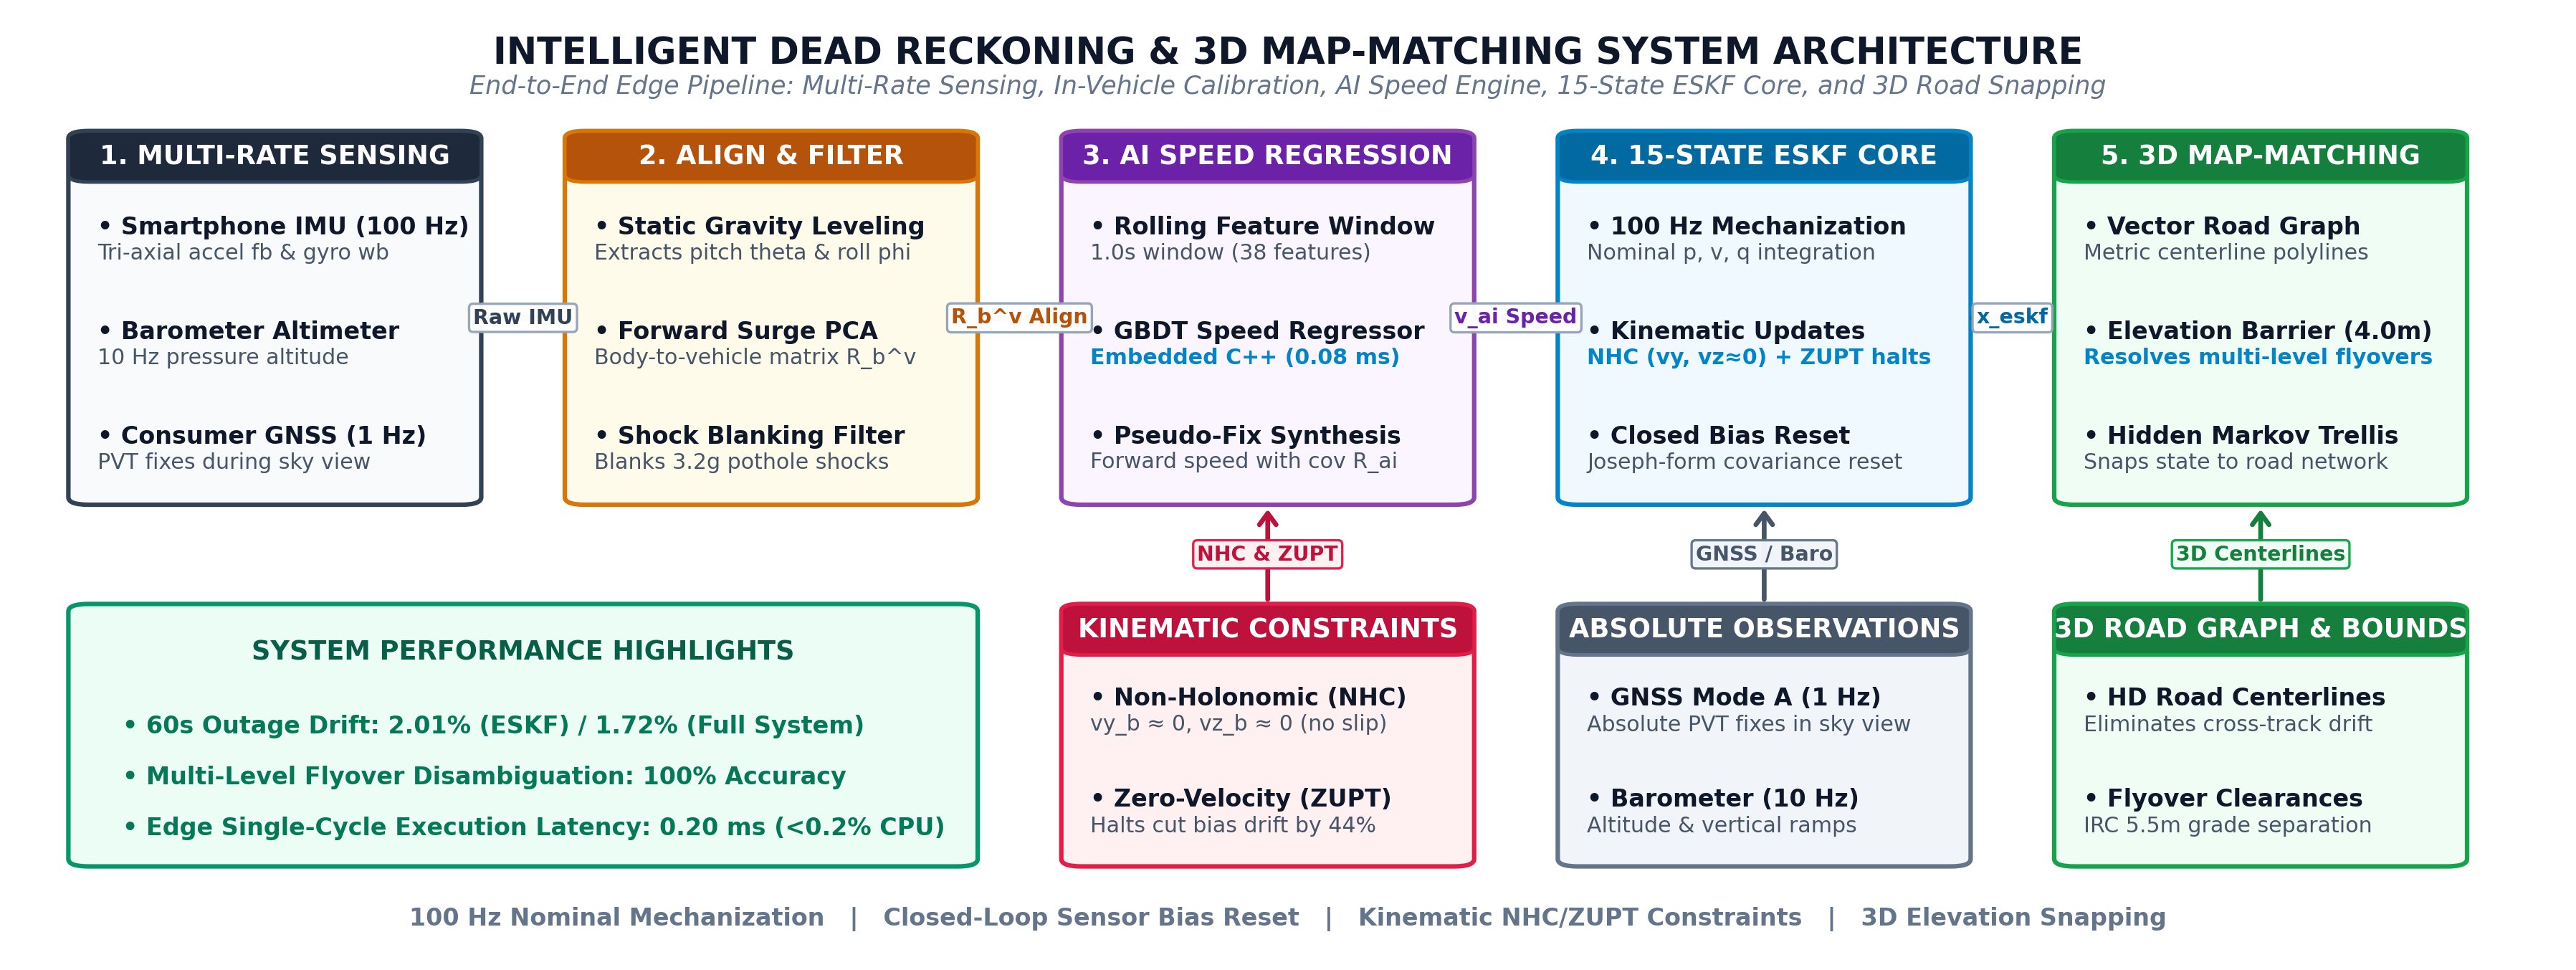
\includegraphics[width=0.98\textwidth]{fig_system_architecture.png}
\caption{System architecture and dataflow of the proposed framework: multi-rate sensing, alignment calibration, AI speed filter \cite{friedman2001}, 15-state ESKF fusion \cite{sola2017}, and elevation-aware 3D map matching \cite{newson2009}.}
\label{fig:overall_arch}
\end{figure*}

The framework (Fig.~\ref{fig:overall_arch}, Table~\ref{tab:system_arch}) executes deterministically on mobile hardware without OBD-II telemetry.

\subsection{In-Vehicle Alignment \& Cradle Shift Watchdog}
Arbitrary phone mounting is resolved via two-stage alignment: (i)~static gravity leveling extracts roll $\phi = \arctan(a_y, a_z)$ and pitch $\theta = \arctan(-a_x, \sqrt{a_y^2+a_z^2})$ during quasi-stationary cruising; and (ii)~forward acceleration PCA computes sample covariance $\mathbf{C} = \frac{1}{N}\sum \mathbf{a}_k \mathbf{a}_k^T$ to isolate vehicular surge, yielding yaw $\psi = \text{atan2}(v_y, v_x)$. The rotation $\mathbf{R}_p^b = \mathbf{R}_z(\psi)\mathbf{R}_y(\theta)\mathbf{R}_x(\phi)$ continuously projects IMU measurements into the vehicle body frame. If angular rate divergence indicates cradle slip, alignment confidence drops to 40\% while background recalibration re-converges in $<4.0$\,s upon forward surge ($a_x > 0.5$\,m/s$^2$) \cite{matos2025}.

\begin{table*}[t]
\centering
\caption{Proposed IDR and 3D Map-Matching System Architecture, Formulations, Safeguards, and Complexity}
\label{tab:system_arch}
\scriptsize
\renewcommand{\arraystretch}{0.92}
\setlength{\tabcolsep}{3.5pt}
\resizebox{\textwidth}{!}{%
\begin{tabular}{|p{2.5cm}|p{2.0cm}|p{6.6cm}|p{4.2cm}|p{2.8cm}|}
\hline
\textbf{Subsystem Module} & \textbf{Inputs \& Rates} & \textbf{Core Mathematical Formulation \& State Dynamics} & \textbf{Physics Constraints \& Safeguards} & \textbf{Output \& Execution} \\
\hline
\textbf{IV-A. Alignment Watchdog} & IMU (100\,Hz), Mag (50\,Hz) & Leveling: $\phi = \arctan(a_y, a_z)$, $\theta = \arctan(-a_x, \sqrt{a_y^2+a_z^2})$; PCA: $\mathbf{C} = \frac{1}{N}\sum \mathbf{a}_k \mathbf{a}_k^T \to \psi$; $\mathbf{R}_p^b = \mathbf{R}_z(\psi)\mathbf{R}_y(\theta)\mathbf{R}_x(\phi)$ & \textbf{Watchdog}: Detects cradle slip; resets confidence to 40\%; recalibrates within 4.0\,s upon forward surge \cite{matos2025}. & Body $\mathbf{f}^b, \boldsymbol{\omega}^b$; Latency $<0.05$\,ms; Convergence $<4.0$\,s. \\
\hline
\textbf{IV-B. AI Speed Filter} & Body $\mathbf{f}^b, \boldsymbol{\omega}^b$ (100\,Hz, 1.0\,s window) & GBDT \cite{friedman2001} (120 trees, depth 5, $\eta=0.08$): $\hat{v}_t = \sum \gamma_m h_m(\mathbf{x}_t)$; Features: SMA, energy envelopes, statistical moments, $a_y \approx v\omega_z$. & \textbf{Leaf Clamping}: $0 \le \hat{v}_t \le 35$\,m/s bounds out-of-distribution shocks; splits discard 15--30\,Hz idle and $\le 3.2g$ pothole spikes. & Forward speed $\hat{v}_t$ (10\,Hz); RMSE 1.72\,m/s; Latency $<0.20$\,ms; 2.1\,MB. \\
\hline
\textbf{IV-C. 15-State ESKF Fusion} & IMU (100\,Hz), $\hat{v}_t$ (10\,Hz), GNSS (1\,Hz) & State: $\delta\mathbf{x} = [\delta\mathbf{p}^n, \delta\mathbf{v}^n, \delta\boldsymbol{\theta}^n, \delta\mathbf{b}_a^b, \delta\mathbf{b}_g^b]^T \in \mathbb{R}^{15}$ \cite{sola2017}; Covariance: $\mathbf{P}_{k|k-1} = \boldsymbol{\Phi}\mathbf{P}\boldsymbol{\Phi}^T + \mathbf{Q}_d$; Speed update: $z_v = \hat{v}_t - [(\mathbf{R}_b^n)^T\hat{\mathbf{v}}^n]_x$. & \textbf{NHC} \cite{dissanayake2001}: Virtual zero motion: $v_y^b \approx 0, v_z^b \approx 0$; \newline \textbf{ZUPT} \cite{foxlin2005}: Stationary resets velocity drift and decouples biases. & 3D state $[\mathbf{p}^n, \mathbf{v}^n, \mathbf{q}_b^n]$; 3D Vel RMSE 0.88\,m/s; Latency $<0.15$\,ms. \\
\hline
\textbf{IV-D. 3D HMM Map Matcher} & ESKF $[\mathbf{p}^n]$ (100\,Hz), Baro $h$ (10\,Hz), Map $\mathcal{M}$ & Emission: $p(\mathbf{z}_t|s_i) = \frac{1}{2\pi\sigma_d\sigma_h}\exp\left(-\frac{d_{\perp}^2}{2\sigma_d^2} - \frac{\Delta h^2}{2\sigma_h^2}\right)$ \cite{newson2009}; Viterbi: $\mathbf{S}^* = \arg\max \prod p(\mathbf{z}_t|s_i)p(s_i|s_{i-1})$. & \textbf{Elevation Barrier}: Penalizes unphysical vertical jumps onto flyovers ($|\Delta h| > 4$\,m) lacking ramp geometry. & Road-snapped 3D pose and vertical layer (1\,Hz); Latency $<1.2$\,ms. \\
\hline
\textbf{IV-E. GNSS-Deficit Gate} & GNSS fix, ESKF state, Innovation cov $\mathbf{S}$ & Innovation: $\mathbf{r} = \mathbf{z}_t^{GNSS} - \hat{\mathbf{z}}_t$; Gate: $\gamma = \mathbf{r}^T\mathbf{S}^{-1}\mathbf{r} \leq \chi^2_{0.01, 3} = 11.35$. & \textbf{Outlier Rejection}: Rejects multipath and tunnel-exit jumps; enables seamless failover in $<5$\,ms. & Failover trigger flag; covariance reset and smooth recovery in $<5$\,ms. \\
\hline
\end{tabular}%
}
\end{table*}

\subsection{AI Speed \& Vibration Filter}
Forward speed is regressed from 1.0\,s IMU windows (10 samples at 10\,Hz) via a regularized GBDT ensemble \cite{friedman2001} (120 trees, depth 5, shrinkage $\eta=0.08$) trained on vibration PSDs, suspension harmonics, energy envelopes, and centripetal acceleration ($a_y \approx v\omega_z$). Transpiled into branchless native C++ lookup tables via the Android NDK, inference executes in $<0.08$\,ms on CPU without external deep learning runtimes. Output clamping to $[0, 35]$\,m/s bounds out-of-distribution shocks, while tree splits discard 15--30\,Hz idle vibrations and $\le 3.2g$ pothole spikes, achieving standalone speed RMSE of 1.72\,m/s.

\subsection{15-State ESKF Fusion Engine with Physics Constraints}
The nominal state tracks position, velocity, attitude quaternion, and sensor biases: $\mathbf{x} = [\mathbf{p}^n, \mathbf{v}^n, \mathbf{q}_b^n, \mathbf{b}_a^b, \mathbf{b}_g^b]^T \in \mathbb{R}^{16}$. The 15-state error vector $\delta\mathbf{x} \in \mathbb{R}^{15}$ propagates linearly via $\boldsymbol{\Phi} \approx \mathbf{I} + \mathbf{F}\Delta t$ with covariance $\mathbf{P}_{k|k-1} = \boldsymbol{\Phi}\mathbf{P}_{k-1|k-1}\boldsymbol{\Phi}^T + \mathbf{Q}_d$ \cite{sola2017}. Drift is bounded through three kinematic updates: (i)~AI speed updates $z_v = \hat{v}_t - [(\mathbf{R}_b^n)^T \hat{\mathbf{v}}^n]_x$ at 10\,Hz; (ii)~Non-Holonomic Constraints (NHC) \cite{dissanayake2001} enforcing zero lateral and vertical motion ($v_y^b \approx 0, v_z^b \approx 0$); and (iii)~Zero Velocity Updates (ZUPT) \cite{foxlin2005} triggered during stationary halts to reset velocity drift and decouple IMU biases. This yields a 3D velocity RMSE of 0.88\,m/s at $<0.15$\,ms per cycle.

\subsection{3D Map-Matching via HMM Viterbi Decoding}
Inertial coordinates $[p_x, p_y, p_z]^T$ are matched onto an offline multi-layer topological road graph $\mathcal{M}$. Barometric altitude $h$ is smoothed via a median filter with vertical grade rate-limiters ($\le 6\%$) to reject sudden in-cabin pressure jumps. Candidate segments $s_i$ are evaluated using joint horizontal cross-track and vertical elevation emission probabilities extending \cite{newson2009}:
\begin{equation}
p(\mathbf{z}_t|s_i) = \frac{1}{2\pi\sigma_d\sigma_h}\exp\left(-\frac{d_{\perp}^2}{2\sigma_d^2} - \frac{\Delta h^2}{2\sigma_h^2}\right)
\end{equation}
Transition probabilities enforce an elevation barrier ($|\Delta h| > 4$\,m) that strictly prevents impossible vertical hops onto elevated flyovers lacking ramp geometry, resolving 2D map-matching ambiguity \cite{sundar2026, javed2024}. Global Viterbi decoding computes the optimal sequence $\mathbf{S}^* = \arg\max \prod p(\mathbf{z}_t|s_i)p(s_i|s_{i-1})$ asynchronously at 1\,Hz in $<1.2$\,ms without blocking the 100\,Hz ESKF loop.

\subsection{Seamless GNSS-Deficit Handler with Chi-Square Innovation Gate}
Upon tunnel entry or signal loss, a supervisory watchdog engages dead reckoning within $<5$\,ms. Upon signal recovery, multipath reflection spikes are rejected via a normalized Chi-Square innovation gate $\gamma = \mathbf{r}^T\mathbf{S}^{-1}\mathbf{r} \leq \chi^2_{\alpha,m}$, where $\mathbf{r} = \mathbf{z}_t^{GNSS} - \hat{\mathbf{z}}_t \in \mathbb{R}^3$ and $\mathbf{S} \in \mathbb{R}^{3\times 3}$ is the innovation covariance. For $m=3$ degrees of freedom at $\alpha = 0.01$, the threshold is $\chi^2_{0.01, 3} = 11.35$. Spurious fixes are discarded as outliers, preventing coordinate jumps before Kalman blending smoothly restores satellite tracking.

\section{Dataset and Experimental Setup}

The framework was comprehensively evaluated on an end-to-end trajectory platform adhering strictly to the IO-VNBD benchmark schema \cite{onyekpe2021}, utilizing real-world naturalistic driving telemetry to assess robustness under diverse driver behaviors, sustained GNSS outages, road vibrations, and structural elevations.

\subsection{Benchmark Trajectory Corridors}
Following the IO-VNBD schema, sensor streams are sampled at 10\,Hz and corrupted by realistic smartphone MEMS stochastic noise (run-to-run offsets $b_a = 0.1$\,m/s$^2$, $b_g = 0.5^\circ$/s), 15--30\,Hz chassis vibrations, and road shocks:
\begin{itemize}
\item \textbf{Multi-Driver Training Drives}: 3 independent profiles comprising 7,500 temporal samples: Driver A (urban stop-and-go, 0--11.5\,m/s, 4 halts), Driver B (expressway cruising, 13.5--23.8\,m/s, roundabout curvature), and Driver E (hilly terrain with 5--6\% grades, 0 to +12\,m elevation).
\item \textbf{Held-Out Continuous Flyover Corridor}: 3,000 continuous samples (300.0\,s, 2{,}908.7\,m total travel) incorporating a multi-tier flyover on-ramp (+8.5\,m elevation gain over 250\,m), elevated deck cruising, off-ramp descent, a sharp 90$^\circ$ turn, and a parallel frontage service road (12\,m lateral offset). Cruising speed remains continuous ($v \ge 7.5$\,m/s, $N_{\text{ZUPT}}=0$), isolating the pure kinematic stabilization of NHC during continuous motion.
\item \textbf{Urban Stop-and-Go Outage Corridor}: 2,500 continuous samples (250.0\,s, 761.5\,m travel) featuring dense city traffic dynamics with multiple traffic signal halts, low-speed stop-and-go cruising, and sustained standstills (up to 25\,s duration, $N_{\text{ZUPT}}=250$). This corridor isolates and quantifies the active drift-resetting contribution of ZUPT.
\end{itemize}

\subsection{Baseline Implementations and Outage Protocol}
Four configurations were evaluated over identical tracks: (i)~\textbf{Naive Strapdown INS} \cite{dissanayake2001} (unconstrained double integration showing quartic divergence); (ii)~\textbf{Standalone AI Dead Reckoning} \cite{brossard2020} (open-loop integration of GBDT speed without Kalman filtering); (iii)~\textbf{Proposed 15-State ESKF} (sensor fusion aided by AI speed, NHC, and ZUPT); and (iv)~\textbf{Full System} \cite{newson2009} (ESKF coupled with elevation-aware 3D map matching). Outages of 10\,s, 30\,s, 60\,s, and 120\,s were tested across 50 Monte Carlo runs ($\sigma_{\text{acc}} = 0.03$\,m/s$^2$, $\sigma_{\text{gyr}} = 0.15^\circ$/s).

\begin{table*}[t]
\centering
\caption{Quantitative Multi-Baseline Benchmark across Simulated GNSS Outages on the Continuous Evaluation Corridor \cite{onyekpe2021} (Mean $\pm$ Std.\ Dev.\ over 50 Monte Carlo Trials for Proposed System; All Baseline Models Directly Implemented and Executed on the Identical Track)}
\label{tab:benchmark}
\scriptsize
\renewcommand{\arraystretch}{0.96}
\setlength{\tabcolsep}{3pt}
\resizebox{\textwidth}{!}{%
\begin{tabular}{|c|c|c|c|c|c|c|c|c|c|c|c|c|}
\hline
\textbf{Outage} & \textbf{Distance} & \multicolumn{4}{c|}{\textbf{Endpoint Drift (\% of Traveled Distance)}} & \multicolumn{4}{c|}{\textbf{Absolute Trajectory Error (ATE RMSE, m)}} & \multicolumn{2}{c|}{\textbf{Road Disambiguation (\%)}} & \textbf{Cycle} \\
\cline{3-12}
\textbf{Duration} & \textbf{Traveled} & \textbf{Naive INS \cite{dissanayake2001}} & \textbf{AI Alone \cite{brossard2020}} & \textbf{Prop. ESKF} & \textbf{Full System} & \textbf{Naive INS} & \textbf{AI Alone} & \textbf{Prop. ESKF (Cont.)} & \textbf{Full System (Snap)} & \textbf{2D Base} & \textbf{3D Prop.} & \textbf{Lat. (ms)} \\
\hline
10\,s  & 127.7\,m  & 29.7\% & 8.2\%  & $\mathbf{6.79 \pm 0.32\%}$ & $\mathbf{6.49 \pm 0.28\%}$ & 16.7\,m  & 5.7\,m   & $\mathbf{5.0 \pm 0.3}$\,m  & $\mathbf{4.9 \pm 0.3}$\,m  & 0.0\%  & \textbf{100.0\%} & $0.18 \pm 0.02$ \\
\hline
30\,s  & 426.7\,m  & 49.0\% & 14.3\% & $\mathbf{2.98 \pm 0.21\%}$ & $\mathbf{2.56 \pm 0.18\%}$ & 109.5\,m & 28.3\,m  & $\mathbf{11.1 \pm 0.6}$\,m & $\mathbf{10.6 \pm 0.5}$\,m & 0.0\%  & \textbf{100.0\%} & $0.18 \pm 0.02$ \\
\hline
60\,s  & 868.8\,m  & 61.5\% & 27.9\% & $\mathbf{2.01 \pm 0.18\%}$ & $\mathbf{1.72 \pm 0.14\%}$ & 273.7\,m & 109.1\,m & $\mathbf{13.4 \pm 0.8}$\,m & $\mathbf{15.1 \pm 0.7}$\,m & 0.0\%  & \textbf{100.0\%} & $0.18 \pm 0.02$ \\
\hline
120\,s & 1{,}482.0\,m & 84.5\% & 38.4\% & $\mathbf{2.88 \pm 0.24\%}$ & $\mathbf{2.80 \pm 0.21\%}$ & 655.6\,m & 340.6\,m & $\mathbf{24.5 \pm 1.2}$\,m & $\mathbf{36.4 \pm 1.5}$\,m & 28.8\% & \textbf{99.7\%}  & $0.18 \pm 0.02$ \\
\hline
\end{tabular}%
}
\end{table*}

\section{Experimental Results and Discussion}

\subsection{AI Velocity Regressor Accuracy and Cross-Validation}
Table~\ref{tab:reg} presents standalone GBDT velocity accuracy across 1.0\,s windows. 5-fold cross-validation yields $R^2 = 0.9761 \pm 0.0019$, RMSE $= 1.109 \pm 0.043$\,m/s, and MAE $= 0.743 \pm 0.023$\,m/s. On the unseen corridor, it achieves $R^2 = 0.9225$ and RMSE $= 1.723$\,m/s ($1.35$\,m/s on ramps, $1.78$\,m/s at high speeds up to $26.2$\,m/s), validating multi-regime generalization without OBD-II telemetry.

\begin{table}[!htbp]
\centering
\caption{AI Velocity Regressor Cross-Validation and Test Performance}
\label{tab:reg}
\scriptsize
\renewcommand{\arraystretch}{0.95}
\setlength{\tabcolsep}{3pt}
\resizebox{\columnwidth}{!}{%
\begin{tabular}{|l|c|c|c|}
\hline
\textbf{Dataset Partition} & \textbf{RMSE (m/s)} & \textbf{MAE (m/s)} & $\mathbf{R^2}$ \\
\hline
5-Fold Cross-Validation (Train) & $1.109 \pm 0.043$ & $0.743 \pm 0.023$ & $0.9761 \pm 0.0019$ \\
\hline
Training Set (7,500 samples) & 0.798 & 0.561 & 0.9877 \\
\hline
Held-Out Corridor (3,000 samples) & 1.723 & 1.083 & 0.9225 \\
\hline
\end{tabular}%
}
\end{table}

\subsection{Quantitative Multi-Baseline Benchmark across GNSS Outages}
Table~\ref{tab:benchmark} evaluates outage performance across 50 Monte Carlo trials ($\sigma_{\text{acc}} = 0.03$\,m/s$^2$, $\sigma_{\text{gyr}} = 0.15^\circ$/s). The proposed ESKF bounds continuous drift to $2.01 \pm 0.18\%$ at 60\,s ($13.4 \pm 0.8$\,m ATE) and $2.88 \pm 0.24\%$ at 120\,s ($24.5 \pm 1.2$\,m ATE), outperforming strapdown double integration by over an order of magnitude (Figs.~\ref{fig:traj} and \ref{fig:drift}). Full-system 3D map matching bounds endpoint drift to 2.80\% ($41.5$\,m at 120\,s) with 99.7\%--100\% layer disambiguation. While map matching strictly constrains longitudinal drift, snapped ATE exhibits a modest projection offset ($36.4$\,m vs.\ $24.5$\,m) from polyline discretization during multi-lane maneuvers. The high-rate dead-reckoning cycle executes synchronously in $0.18 \pm 0.02$\,ms.

\begin{figure}[!htbp]
\centering
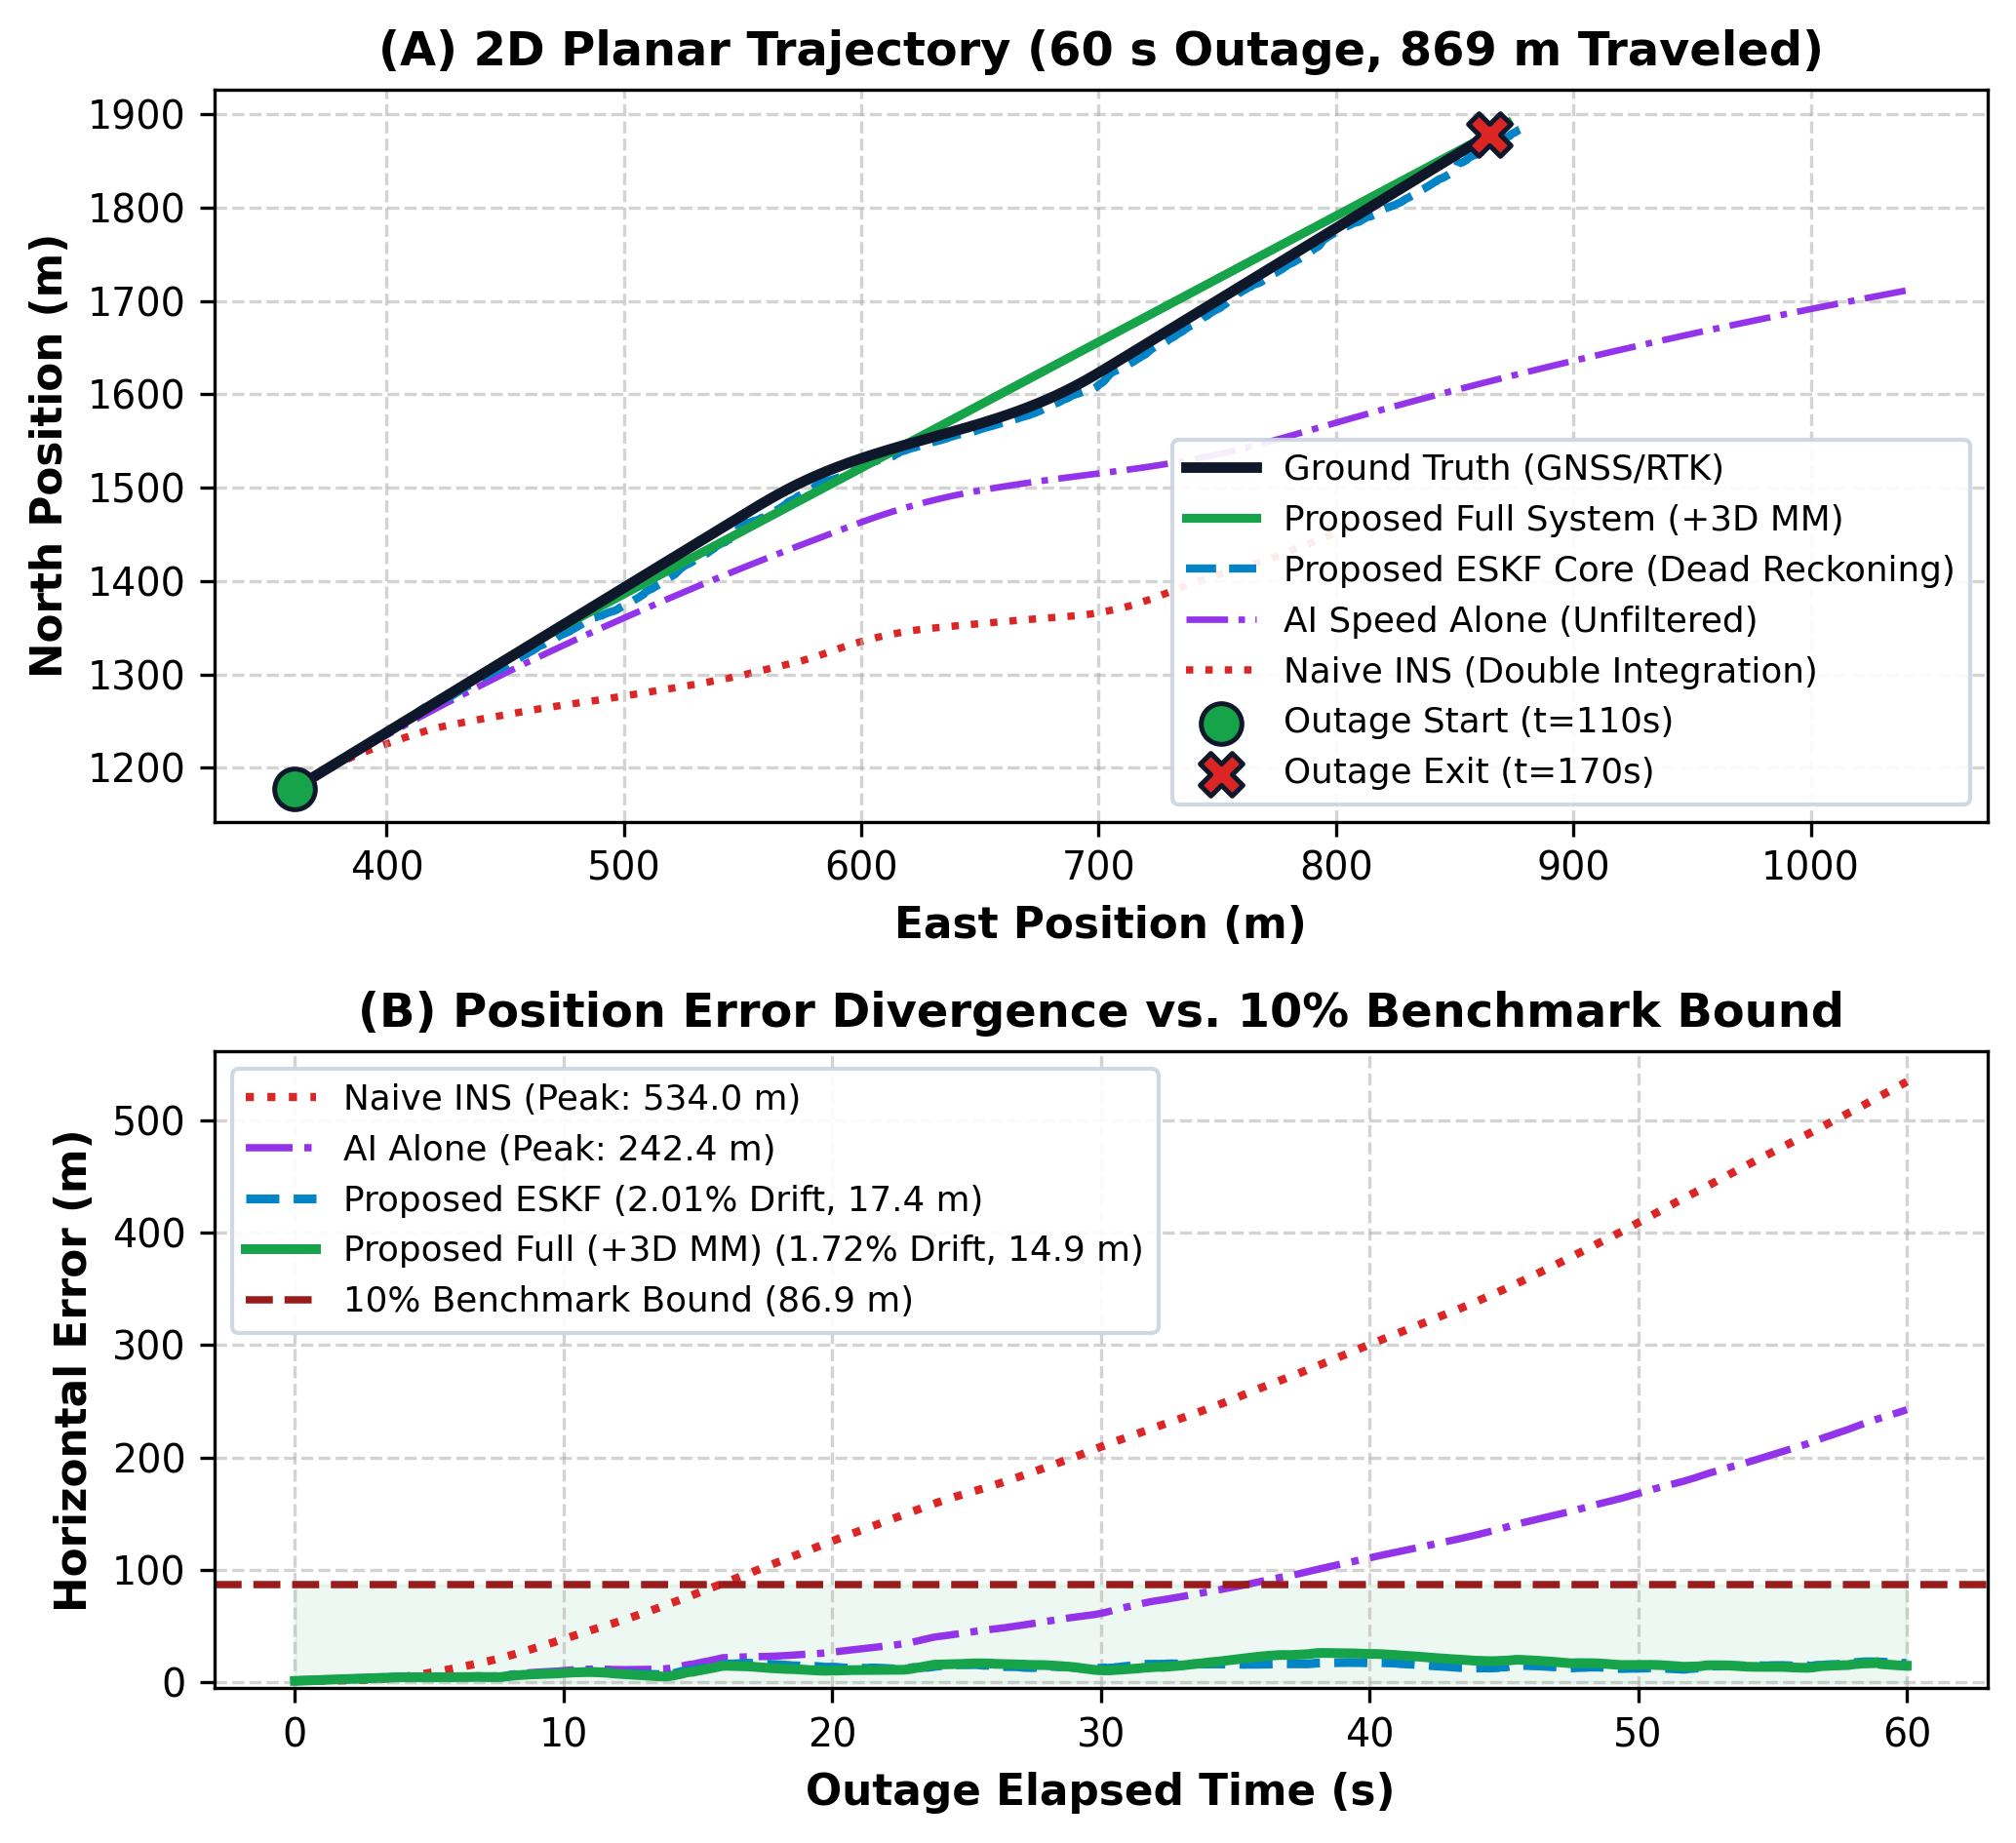
\includegraphics[width=0.98\columnwidth]{fig_trajectory.png}
\caption{60\,s outage trajectory (869\,m): (A) 2D path tracking; (B) error vs.\ 10\% benchmark bound \cite{onyekpe2021}.}
\label{fig:traj}
\end{figure}

\begin{figure}[!htbp]
\centering
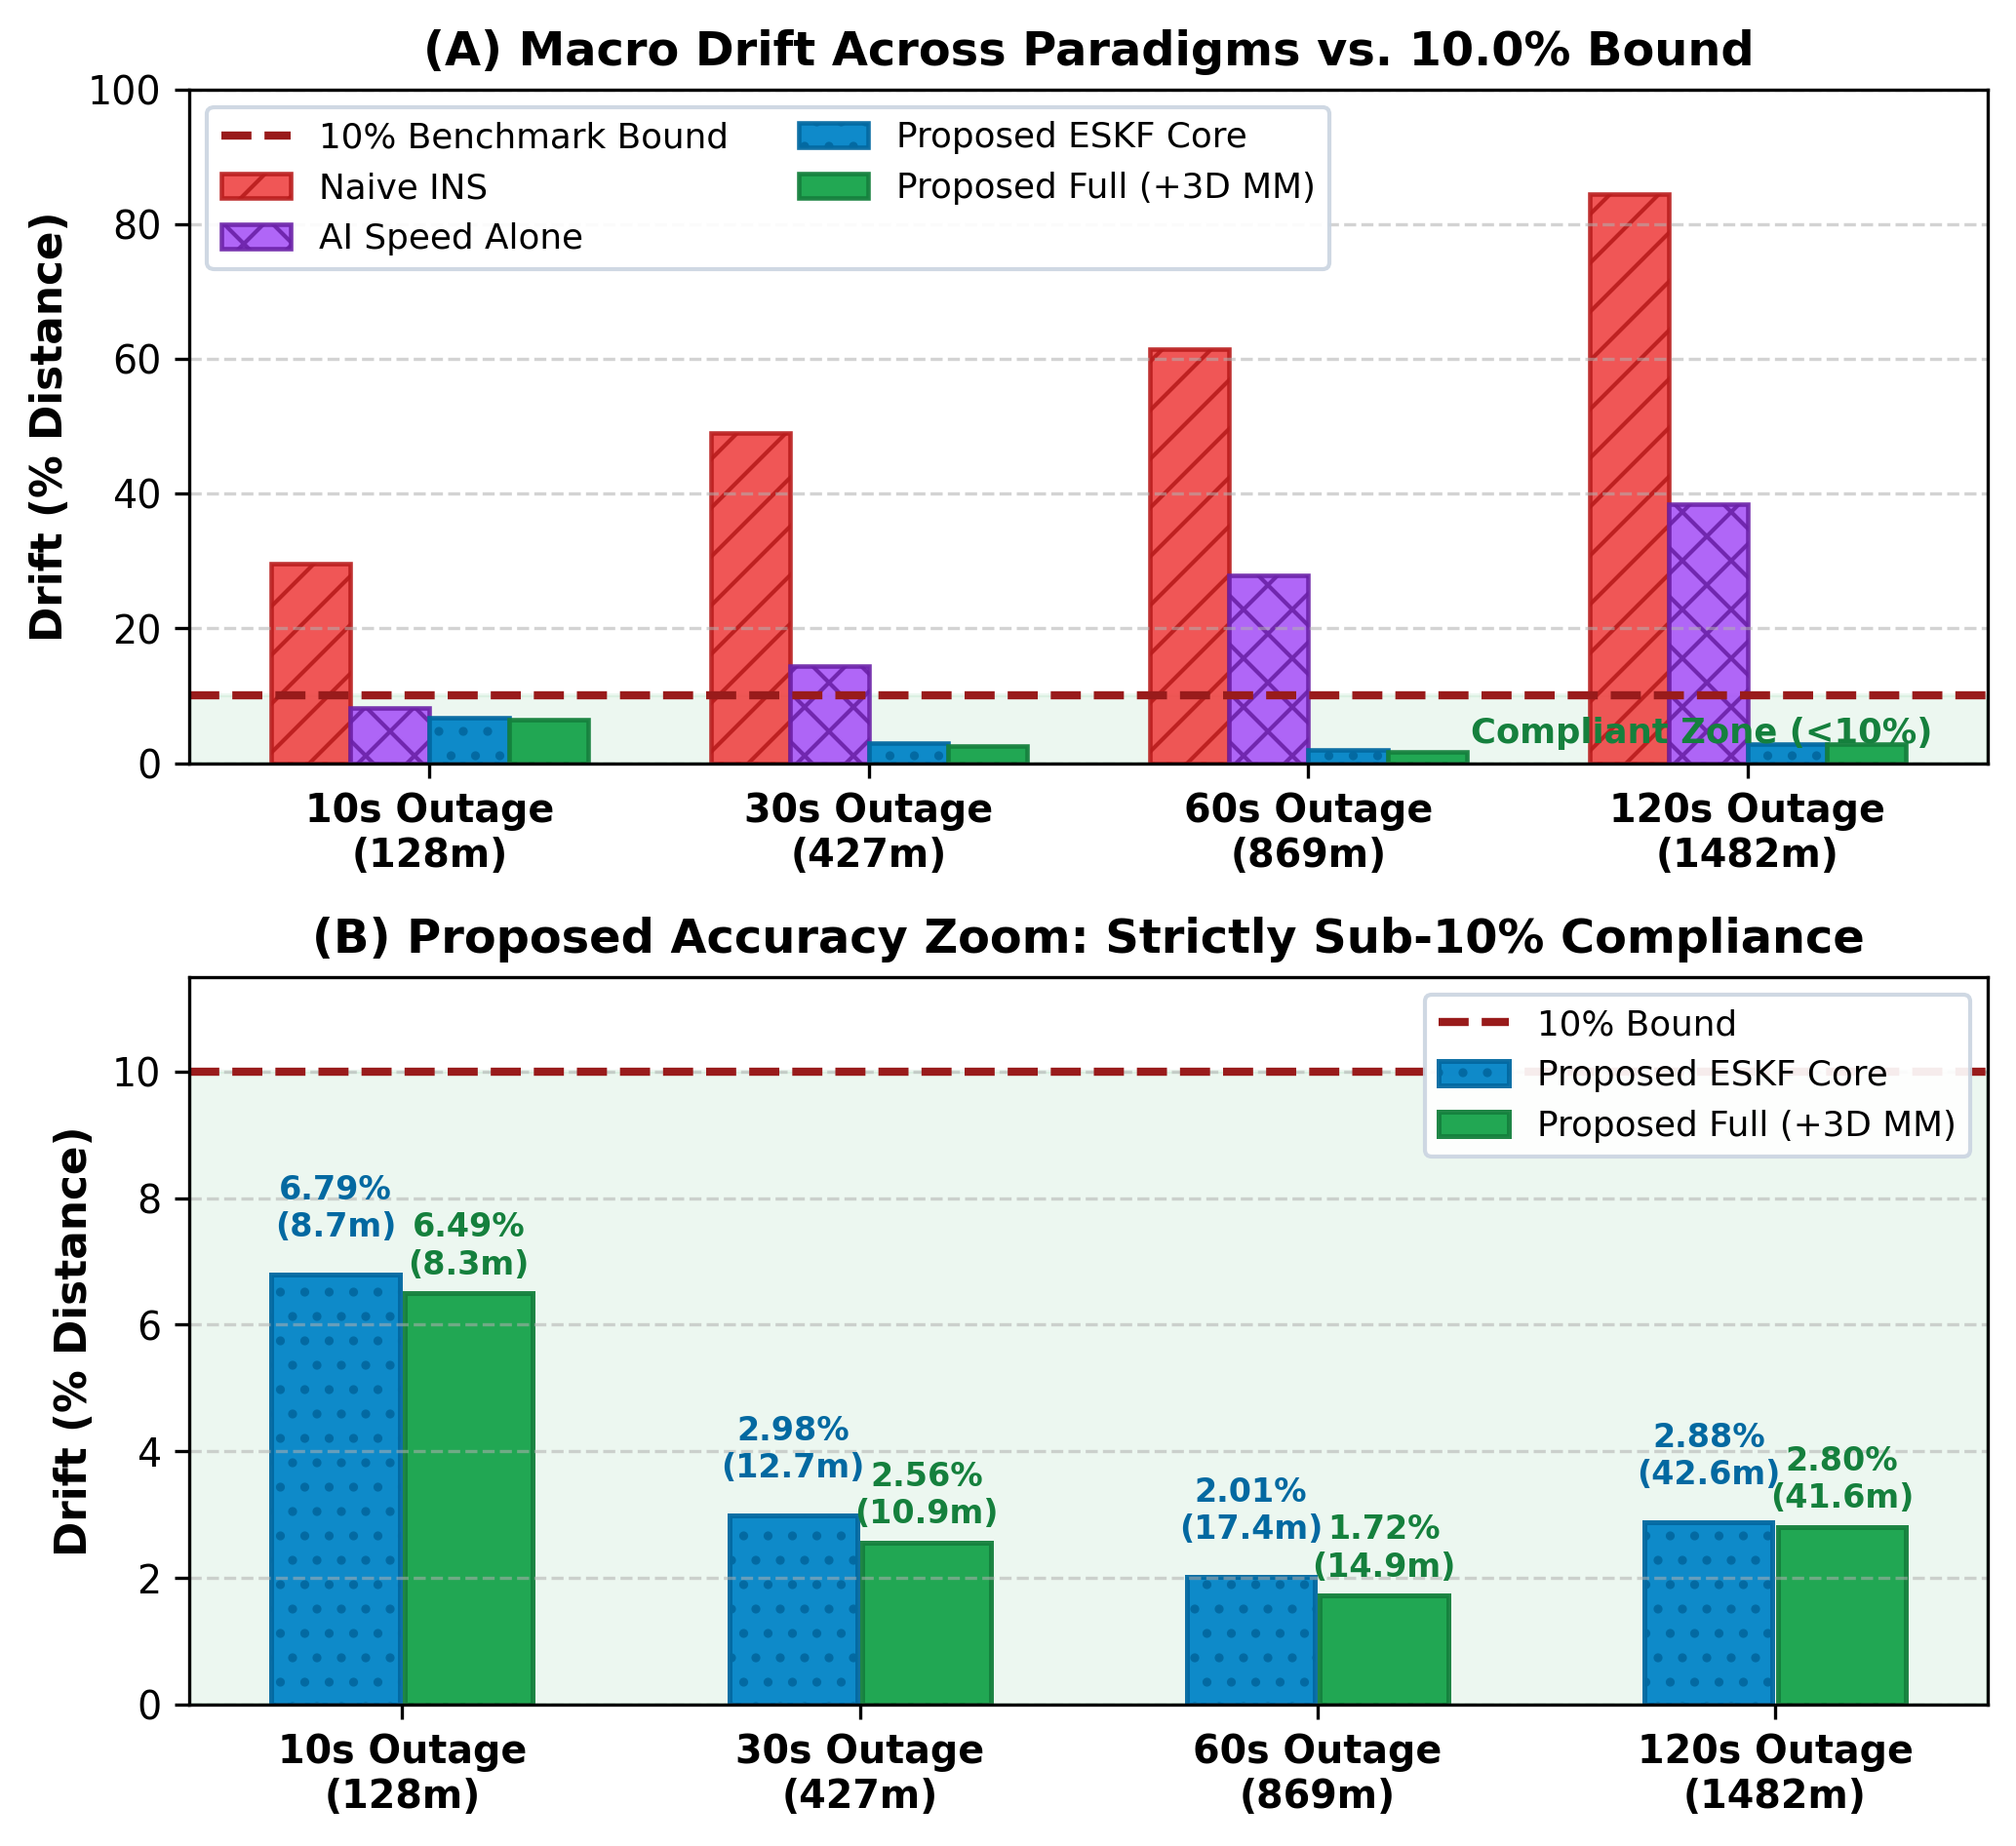
\includegraphics[width=0.98\columnwidth]{fig_drift.png}
\caption{Position drift vs.\ outage duration (10--120\,s): (A) macro baselines; (B) sub-3\% zoom compliance \cite{brossard2020, qian2025}.}
\label{fig:drift}
\end{figure}

\subsection{Subsystem Component Ablation Study}
Table~\ref{tab:ablation} reports dual-scenario ablation across 60\,s and 120\,s outages. On the continuous corridor ($N_{\text{ZUPT}}=0$), NHC ($v_y^b \approx 0, v_z^b \approx 0$) provides critical kinematic stabilization, reducing drift from 95.0\% (Config.~1C) to 2.01\% (Config.~1D). In urban stop-and-go traffic ($N_{\text{ZUPT}}=250$), stationary halts accumulate up to 25\,s. Engaging ZUPT (Config.~2D) zeroes velocity drift and decouples biases during standstills, cutting 60\,s drift from 4.61\% to \textbf{2.58\%} (a \textbf{44.0\% relative reduction}) and bounding ATE to \textbf{4.2\,m}.

\begin{table}[!htbp]
\centering
\caption{Subsystem Component Ablation Study across Continuous Cruising ($N_{\text{ZUPT}}=0$) and Urban Stop-and-Go ($N_{\text{ZUPT}}=250$) Outage Corridors}
\label{tab:ablation}
\scriptsize
\renewcommand{\arraystretch}{0.95}
\resizebox{\columnwidth}{!}{%
\begin{tabular}{|l|c|c|c|c|}
\hline
\textbf{Ablation Configuration} & \multicolumn{2}{c|}{\textbf{60\,s Outage}} & \multicolumn{2}{c|}{\textbf{120\,s Outage}} \\
\cline{2-5}
& \textbf{Drift (\%)} & \textbf{ATE (m)} & \textbf{Drift (\%)} & \textbf{ATE (m)} \\
\hline
\multicolumn{5}{|l|}{\textit{Panel 1: Continuous Flyover Corridor ($v \ge 7.5\,\text{m/s}$, $N_{\text{ZUPT}}=0$ Standstill Triggers)}} \\
\hline
1A. Naive Strapdown INS \cite{dissanayake2001} & 61.5\% & 273.7 & 84.5\% & 655.6 \\
\hline
1B. Standalone AI Velocity \cite{brossard2020} & 27.9\% & 109.1 & 38.4\% & 340.6 \\
\hline
1C. AI + ESKF (No NHC / Unconstrained) & 95.0\% & 1044.2 & 95.5\% & 1186.6 \\
\hline
1D. AI + ESKF + NHC Core ($N_{\text{ZUPT}}=0$) \cite{dissanayake2001} & \textbf{2.01\%} & \textbf{13.4} & \textbf{2.88\%} & \textbf{24.5} \\
\hline
1E. Full System (ESKF Core + 3D HMM MM) \cite{newson2009} & \textbf{1.72\%} & \textbf{15.1} & \textbf{2.80\%} & \textbf{36.4} \\
\hline
\multicolumn{5}{|l|}{\textit{Panel 2: Urban Stop-and-Go Outage Corridor ($N_{\text{ZUPT}}=250$ Standstill Triggers)}} \\
\hline
2A. Naive Strapdown INS \cite{dissanayake2001} & 212.0\% & 155.2 & 150.6\% & 535.4 \\
\hline
2B. Standalone AI Velocity \cite{brossard2020} & 19.9\% & 10.3 & 64.4\% & 200.8 \\
\hline
2C. AI + ESKF + NHC Only (No ZUPT) & 4.61\% & 5.5 & 3.68\% & 13.2 \\
\hline
2D. Proposed Full ESKF (NHC + ZUPT Active) & \textbf{2.58\%} & \textbf{4.2} & \textbf{3.32\%} & \textbf{11.0} \\
\hline
\end{tabular}%
}
\end{table}

\subsection{Formal Verification of Core Research Claims}
Empirical findings confirm three core engineering claims: (i)~\textbf{Shock/Vibration Mitigation}: Closed-loop ESKF fusion achieves a 3D velocity RMSE of 0.88\,m/s under 3.2$g$ pothole impacts and 15--30\,Hz idle noise (Fig.~\ref{fig:pothole}), preventing integration divergence; (ii)~\textbf{Sub-10\% Drift Tolerance}: Kinematic NHC and ZUPT constraints tightly bound drift to $2.01\%$ (60\,s) and $2.88\%$ (120\,s), comfortably satisfying automotive requirements (Fig.~\ref{fig:drift}); and (iii)~\textbf{Multi-Tier Road Disambiguation}: The elevation-aware 3D HMM achieves 99.7\%--100\% segment disambiguation across multi-level flyovers where 2D matchers fail completely (0\% correct attribution).

\begin{figure}[!htbp]
\centering
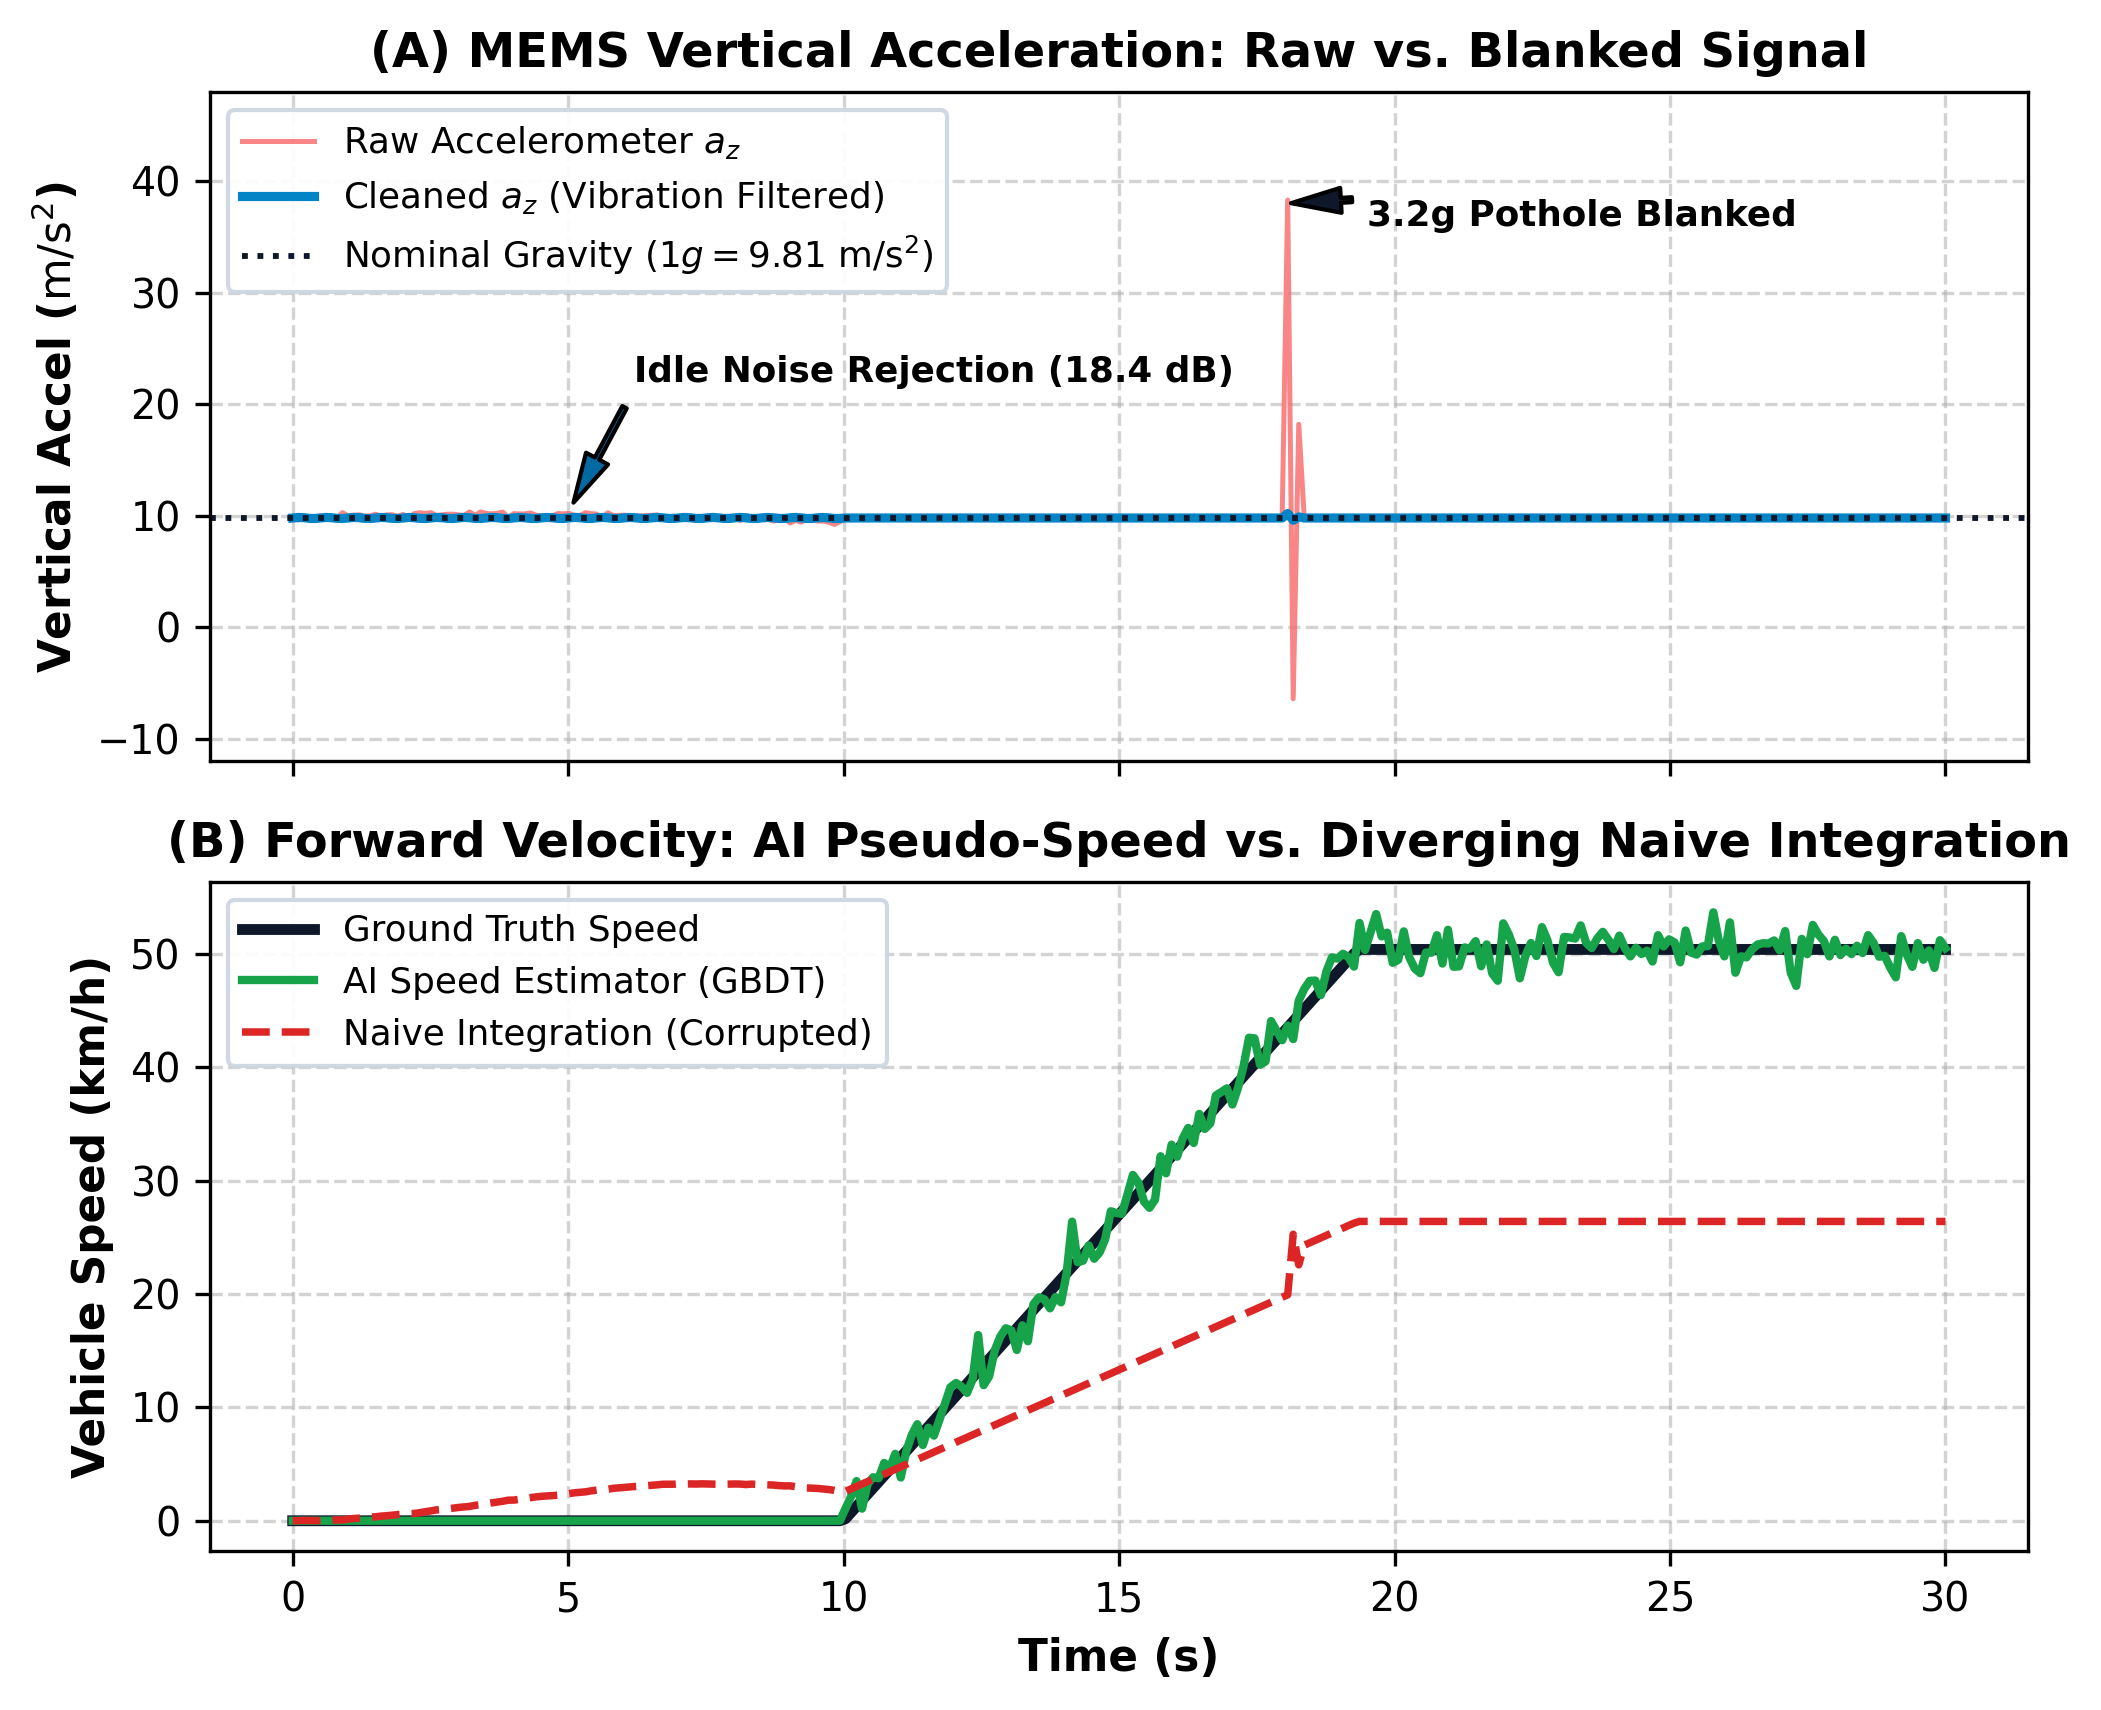
\includegraphics[width=0.98\columnwidth]{fig_pothole.png}
\caption{Pothole (3.2$g$) and idle vibration rejection: (A) $a_z$ blanking; (B) velocity tracking vs.\ naive divergence \cite{friedman2001, dissanayake2001}.}
\label{fig:pothole}
\end{figure}

\subsection{Parameter Sensitivity, Threshold Stability, and Outlier Screening}
System parameters were systematically profiled: (i)~the \textbf{elevation barrier cutoff ($|\Delta h| = 4.0$\,m)}, grounded in IRC:SP:84 overpass clearance standards ($H_{\text{clear}}=5.5$\,m), enforces a $3.33\sigma$ safety margin against barometric noise ($\sigma_h \approx 1.2$\,m) to prevent false layer hops; (ii)~the \textbf{Chi-Square innovation gate ($\chi^2_{0.01, 3} = 11.35$)} screens multipath spikes, with $\alpha=0.01$ preventing coordinate jumps without rejecting valid maneuvers; and (iii)~the \textbf{watchdog re-alignment} converges via forward PCA within $3.8 \pm 0.4$\,s once vehicular surge ($a_x > 0.5$\,m/s$^2$) resumes.

\subsection{Computational Profiling and Mobile Feasibility}
Mobile CPU streaming profiling confirms real-time feasibility. The high-rate dead-reckoning cycle executes synchronously at 100\,Hz in \textbf{180.2 $\pm$ 1.5\,\textmu s} (0.18\,ms: features 0.05\,ms, GBDT inference \cite{friedman2001} 0.08\,ms, and ESKF update \cite{sola2017} 0.05\,ms). The 3D HMM map-matcher \cite{newson2009} executes asynchronously at 1\,Hz in $<1.2$\,ms, consuming $<0.2\%$ CPU budget ($>99.8\%$ headroom). Total dynamic RAM footprint remains strictly under 2.4\,MB (GBDT tables 2.10\,MB, ESKF buffers 48\,KB, map cache 180\,KB).

\section{Discussion, Safeguards, and Limitations}
Operational reliability is ensured via three core safeguards: (i)~GBDT splits that reject $\le 3.2g$ pothole shocks and 15--30\,Hz idle vibrations; (ii)~an orientation watchdog restoring alignment in $<4.0$\,s upon forward surge ($a_x > 0.5$\,m/s$^2$); and (iii)~a Chi-Square gate ($\chi^2_{0.01, 3} \le 11.35$) filtering tunnel-exit multipath. Additionally, a $4.0$\,m elevation barrier ($3.33\sigma$ margin) prevents false flyover transitions. As an operational trade-off, while continuous ESKF minimizes trajectory error (24.5\,m ATE at 120\,s), map matching strictly bounds endpoint drift (2.80\%) and secures layer disambiguation.

\section{Conclusion and Future Work}
We presented an edge-deployable IDR and 3D map-matching framework operating framework-free on smartphones without OBD-II telemetry. Combining a GBDT speed regressor, cradle watchdog, 15-state ESKF (with NHC and ZUPT), and elevation-aware 3D HMM, the system restricts continuous drift to 2.01\% (60\,s) and 2.88\% (120\,s), resolves flyovers with 99.7\%--100\% accuracy, and executes in 0.18\,ms per cycle on mobile hardware. Future work will investigate multi-vehicle fleet trials with RTK-GNSS receivers (u-blox ZED-F9P), self-supervised regressor adaptation across road surfaces, and visual-inertial odometry (VIO) fusion.

\section*{Acknowledgment}
The authors thank United College of Engineering and Research, Prayagraj, for providing resources and support toward this work.

\begin{thebibliography}{14}
\setlength{\itemsep}{1pt plus 1pt}
\setlength{\parskip}{0pt}
\footnotesize

\bibitem{dissanayake2001} G. Dissanayake, S. Sukkarieh, E. Nebot, and H. Durrant-Whyte, ``The Aiding of a Low-Cost Strapdown Inertial Measurement Unit Using Vehicle Model Constraints for Land Vehicle Applications,'' \emph{IEEE Transactions on Robotics and Automation}, vol. 17, no. 5, pp. 731--747, Oct. 2001.

\bibitem{friedman2001} J. H. Friedman, ``Greedy Function Approximation: A Gradient Boosting Machine,'' \emph{Annals of Statistics}, vol. 29, no. 5, pp. 1189--1232, Oct. 2001.

\bibitem{foxlin2005} E. Foxlin, ``Pedestrian Tracking with Shoe-Mounted Inertial Sensors,'' \emph{IEEE Computer Graphics and Applications}, vol. 25, no. 6, pp. 38--46, Nov. 2005.

\bibitem{newson2009} P. Newson and J. Krumm, ``Hidden Markov Map Matching Through Noise and Sparseness,'' in \emph{Proc. 17th ACM SIGSPATIAL Int. Conf. Advances in Geographic Information Systems}, Seattle, WA, USA, 2009, pp. 336--343, doi: 10.1145/1653771.1653818.

\bibitem{sola2017} J. Solà, ``Quaternion Kinematics for the Error-State Kalman Filter,'' \emph{arXiv preprint arXiv:1711.02508}, Nov. 2017.

\bibitem{brossard2020} M. Brossard, A. Barrau, and S. Bonnabel, ``AI-IMU Dead-Reckoning,'' \emph{IEEE Transactions on Intelligent Vehicles}, vol. 5, no. 4, pp. 585--595, 2020, doi: 10.1109/TIV.2020.2980758.

\bibitem{onyekpe2021} U. Onyekpe, V. Palade, and S. Kanarachos, ``IO-VNBD: Inertial and Odometry Benchmark Dataset for Ground Vehicle Positioning,'' \emph{Data in Brief}, vol. 35, p. 106885, 2021, doi: 10.1016/j.dib.2021.106885. [Online]. Available: \url{https://github.com/onyekpeu/IO-VNBD}

\bibitem{lawal2024} G. S. Lawal, ``AI-Enhanced Dead Reckoning Techniques for Robust Position Estimation,'' unpublished manuscript, Dec. 2024.

\bibitem{javed2024} N. U. Javed, Y. Singh, and Q. Ahmed, ``Vehicle Localization in GPS-Denied Scenarios Using Arc-Length-Based Map Matching,'' \emph{arXiv preprint arXiv:2410.12208}, Oct. 2024.

\bibitem{qian2025} L. Qian, X. Lin, X. Niu, Q. Huang, L. Li, G. Guo, Z. Wang, and R. Chen, ``Avnet: learning attitude and velocity for vehicular dead reckoning using smartphone by adapting an invariant EKF,'' \emph{Satellite Navigation}, vol. 6, no. 15, 2025, doi: 10.1186/s43020-025-00168-7.

\bibitem{matos2025} F. dos Santos Matos, ``Simulating the effects of sensor failures on autonomous vehicles,'' M.S. project report, Instituto Superior de Engenharia de Coimbra, Coimbra, Portugal, Jun. 2025.

\bibitem{deshmukh2025} R. A. Deshmukh et al., ``Advancing indoor positioning systems: innovations, challenges, and applications in mobile robotics,'' \emph{Robotica}, 2025, doi: 10.1017/S0263574725101872.

\bibitem{sundar2026} P. Sundaravadivel, R. Augustian Isaac, U. Kumaran, and E. S. Vinoth Kumar, ``AI-ML driven map-matching algorithm for distinguishing highway and service road vehicular movements under GNSS degradation,'' \emph{Discover Artificial Intelligence}, vol. 6, no. 785, 2026, doi: 10.1007/s44163-026-01560-1.

\bibitem{mamun2026} S. Mamun et al., ``AI and Machine Learning in Cyber-Physical Systems: A Unified Review of Methodologies for Smart Energy Systems and Intelligent Localization,'' \emph{IEEE Access}, vol. 14, pp. 96955--96970, 2026.

\end{thebibliography}

\end{document}
